\documentclass[border=3mm,svgnames]{standalone}
\usepackage{tkz-euclide}

\begin{document}
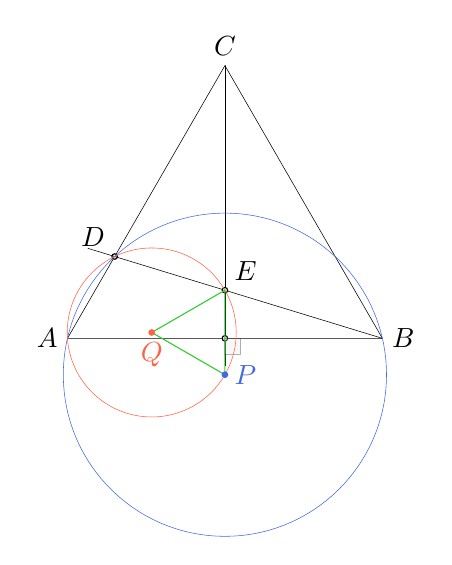
\begin{tikzpicture}
    % set up coordinates
    \tkzDefPoint(0,0){A}
    \tkzDefPoint(4,0){B}
    
    % draw equilateral ABC triangle
    \tkzDefTriangle[equilateral](A,B)\tkzGetPoint{C}
    \tkzDrawPolygon(A,B,C)
    
    % find the intersection of AB with perpendicular line from C
    \tkzDefPointBy[projection=onto A--B](C)\tkzGetPoint{H}
    \tkzDrawLines[add=0 and 0.1](C,H)
    \tkzDrawPoints(H)
    %\tkzMarkRightAngle[size=.2, fill=gray!20, opacity=.3](B,H,C)
    % to mark angle on the outside, get point C' symmetric wrt H
    % suspend the bounding box
    \begin{pgfinterruptboundingbox}
    \tkzDefPointBy[symmetry=center H](C) \tkzGetPoint{C'}
    \tkzMarkRightAngle[size=.2, fill=gray!20, opacity=.3](C',H,B)
    \end{pgfinterruptboundingbox}
    
    % get a point D on line AC
    \tkzDefPointOnLine[pos=0.3](A,C)\tkzGetPoint{D}
    \tkzDrawPoints(D)
    \tkzDrawLines[add=0 and 0.1](B,D)
    
    % get intersection of line BD and CH
    \tkzInterLL(B,D)(C,H)\tkzGetPoint{E}
    \tkzDrawPoints(E)
    %\tkzDrawLines[add=0 and 0.1](A,E)
    
    % first circumcircle
    \tkzDefCircle[circum](A,B,D)\tkzGetPoint{P}
    \tkzDrawCircle[RoyalBlue](P,A)
    
    % second circumcircle
    \tkzDefCircle[circum](A,E,D)\tkzGetPoint{Q}
    \tkzDrawCircle[Tomato](Q,A)
    
    % draw labels
    \tkzLabelPoints[left](A)
    \tkzLabelPoints[right](B)
    \tkzLabelPoints[above](C)
    \tkzLabelPoints[above right](E)
    \tkzLabelPoints[above left](D)
    \tkzLabelPoints[right,RoyalBlue](P)
    \tkzLabelPoints[below,Tomato](Q)
    
   % draw EPQ triangle
   \tkzDrawPolygon[LimeGreen,thin](E,P,Q)
    
    % draw circumcenters
    \tkzDrawPoints[RoyalBlue](P)
    \tkzDrawPoints[Tomato](Q)
    
    % shrink the bounding box
    %\tkzShowBB
    \tkzClipBB
\end{tikzpicture}
\end{document}
